\chapter{Model implementation}
\label{ch:model-implementation}

From all predictors in Table \ref{table:predictors}, only SSRD, STRD, TSR, TP and TCC are used. 
Since the Variables SSRD, STRD and TSR are all available as accumulated fields, they first need to be decumulated.
This can be done by subtracting the value before the current value from the current value, for each day separately. 
Figure \ref{fig:strd-accumulated-vs-decumulated} shows both the accumulated and decumulated fields. 
A machine learning algorithm works better with the decumulated field since the decumulated field directly correlates 
with the power output of the solar plant.

\begin{figure}[h]%
    \centering
    \subfloat[\centering STRD accumulated]{{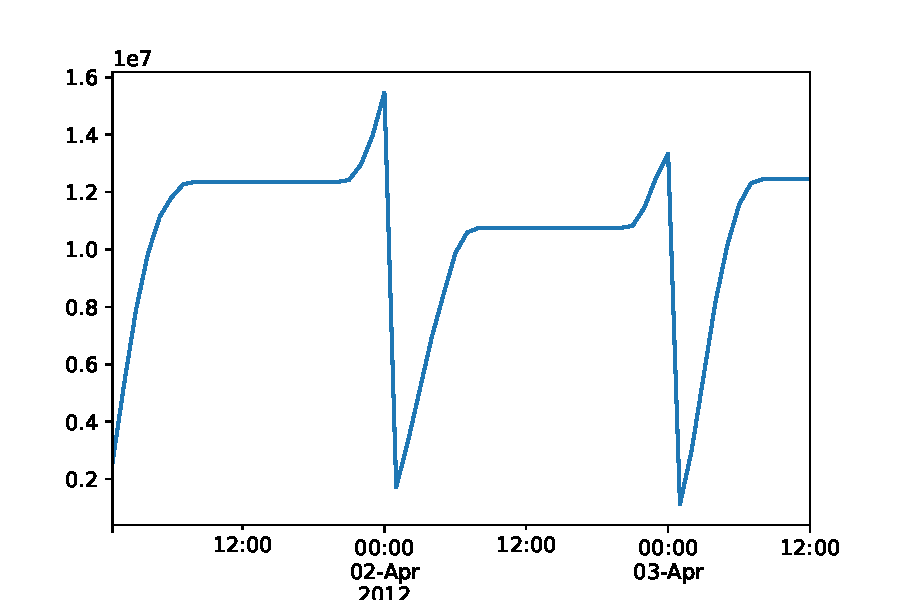
\includegraphics[width=7cm]{plots/strd_accumulated.pdf} }}%
    \qquad
    \subfloat[\centering STRD decumulated]{{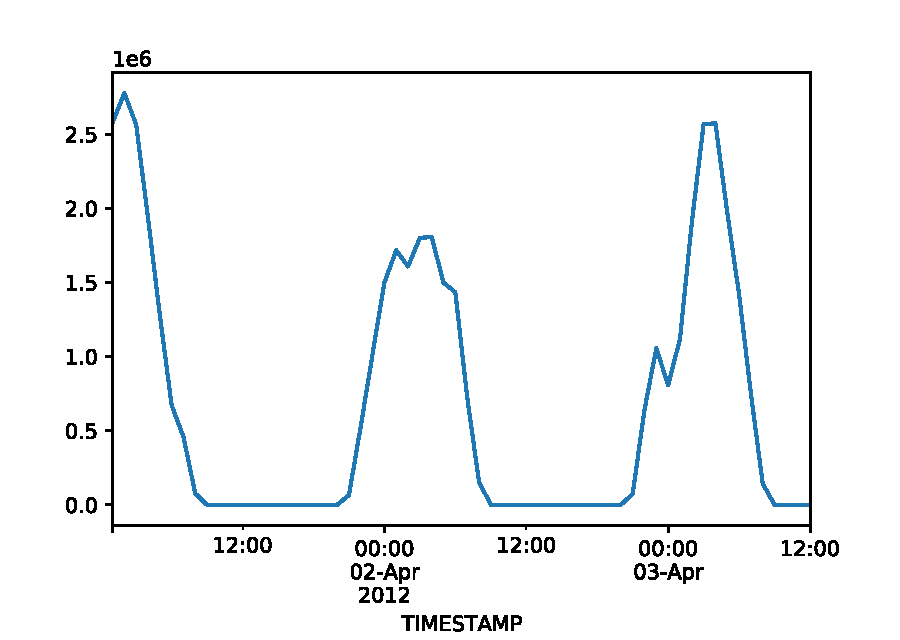
\includegraphics[width=7cm]{plots/strd_decumulated.pdf} }}%
    \caption{STRD accumulated vs. decumulated}%
    \label{fig:strd-accumulated-vs-decumulated}%
\end{figure}

Since we are using some steps like the calculation of the pinball loss, 
it makes sense to use some kind of pipeline structure for the code. 
\Textcite{Heidrich2021} introduced 
pyWATTS\footnote{\url{https://github.com/KIT-IAI/pyWATTS}}: a framework 
that is designed to solve the issue of creating pipelines for time series 
forecasting. 

\section{Spline Quantile Function RNNs}
\label{sec:implementation-sqf-rnn}

The implementation for the SQF-RNN model can be found on GitHub\footnote{\url{https://github.com/awslabs/gluon-ts}}.

The key difference between the SQF-RNN model and the DeepAR model from 
\Textcite{Salinas2017} is that the DeepAR implementation uses a 
probabilistic distribution and optimizes the likelihood of that distribution 
where in the SQF-RNN case spline quantile functions are used and the 
CRPS is optimized. 
For complex problems, the specification on a probabilistic distribution 
that fits the data is often not trivial. 

In the DeepAR default implementation, the Student's \(t\)-distribution is used. 
With this assumption, the model performs noticably worse on the GEFCom14 dataset.

The CRPS is often used to evaluate a forecast model but its usage as 
a direct loss function in the training process is rare. 
As the CRPS is closely related to the pinball loss (see \ref{ch:crps}), 
this helps in the GEFCom14 problem since it directly minimizes the given metric.

First, the data is read from the \texttt{.csv} files. 
After that, the cumulated columns (SSRD, STRD, TSR) are decumulated and then normalized.
Then, the trainig data is converted into a \texttt{ListDataset} and fitted with the 
\texttt{DeepAREstimator} class. The frequency of the model was set to one hour and 
prediction length to 28, 30 or 31 days since the task was to predict one full month. 
In order to use quantile splines with three parts as the output distribution, 
we need to set \texttt{distr\_output=PiecewiseLinearOutput(num\_pieces=3)}. 
Because the default value of \texttt{use\_feat\_dynamic\_real} is set to \texttt{False} 
in the \texttt{DeepAREstimator} model, 
we need to change it to \texttt{True} or else it will ignore the predictors 
\(x_1, \ldots, x_n \in \R^D\). 

After training for seven epochs, the model with the data that is available from the months before, 
we need to predict the upcoming month. This is done by calling the \texttt{predict()} 
method from the predictor that we got after training.
After that, we calculate the quantiles from the prediction and use them to 
calculate the pinball loss for each time step and zone.

In order to get better and more consistent results, the ensemble averaging is used. 
Seven independent models are trained simultaneously and in the predcition step, 
the output of every model is averaged and returned.
\todo{how much performance improvement?}

\section{Nearest Neighbor Quantile Filters}
\label{sec:implementation-nnqf}

The basic steps for the quantile filters are provided by \Textcite{Ordiano2019} 
on GitHub\footnote{\url{https://github.com/JorgeAngel/nnqf_filter}}. 

Since the NNQF method is only a preprocessing step for the target values, 
we still need to decide which model we want to use for fitting the 
conditional distribution function. 
\Textcite{Ordiano2019} tried fitting each of the \(99\) quantiles 
with a polynomial of maximum degree \(1\) to \(4\) or a multi layer perceptron 
with \(6\) or \(10\) hidden neurons. Since the multi layer perceptron leads to 
noticably better results, we will focus on this regression method. 

Because the data is a time series, timepoints that are close are correlated. 
Therefore, we not only take the predictor value \(x_n \in \R^D\) of time point \(n\) 
but also \(x_{n-1}, \ldots, x_{n-H+1}\) as predictor values, where \(H\) is the number of lags.
All in all, we want to fit a function \(\func{f_q}{\R^{D\times H}}{\R}\), 
where \( f(x_n, \ldots, x_{n-H+1}; \theta_{(q)})\) is the conditional 
\(q\)-quantile of the target value \(Y_n\) and \(\theta_{(q)}\) are the weights 
of the regression model for the \(q\)-quantile.

In order to achieve this lagging, pyWATTS contains a \texttt{Sampler} class
that transforms the data in a way that afterwards, each timepoint contains the 
predictor data of the previous \(H\) timepoints.

\Textcite{Ordiano2019} use separate neural networks with \(6\) or \(10\) hidden nodes for each quantile, 
which is computationally more expensive than training one neural network with 
one hidden layer with \(50\) nodes for \(99\) outputs. 
\todo{Both methods perform approximately the same in evaluation chapter; add numbers to show that} 

Since implementing a model in pyWATTS with a variable number of neural networks is currently 
not easily possible, we will use a single neural network to approximate the quantiles.

In order to avoid quantile crossing, \Textcite{Ordiano2019} postprocess the conditional quantiles:
\[ \hat{y}_{(q)} = \begin{cases}
    \max\set{ f(x; \theta_{(q)}), 0 }, &\text{if } q = 0.01, \\
    \max\set{ f(x; \theta_{(q)}), f(x; \theta_{(q-0.01)}) }, &\text{else.}
\end{cases}\]

In this thesis, we use another approach: \\
We sort all estimated conditional quantiles \(\set{ f(x; \theta_{(q)}) \;|\; q\in \set{0.01, \ldots, 0.99} }\) 
and set \(\hat{y}_{(q)}\) as the \((q\cdot 100)\)-th entry of the sorted list. 
\todo{This results in a noticable performance improvement 
in comparison to taking the maximum. add numbers to show noticable improvement! \(\leadsto\) in evaluation chapter}

After that, the pinball loss is calculated the same way as in the QRF case.

In the NNQF model, the only hyperparameters for the preprocessing part are 
the metric that is used calculating the distances, 
the number of neighbors that should be considered and 
the number of lags \(H\). 
The other hyperparameters depend on the regression model. 
In the case of the multi layer perceptron, the usual hyperparameters like 
hidden layer sizes, activation function, solver and learning rate can be tuned. 
To improve stability, we also use ensemble training at the expense of training and evaluation time.
The parameters after tuning as well as the hyperparameter space 
are shown in Table \ref{table:nnqf-hyperparameters}. 
The resulting losses are all in the range \([0.02, 0.025]\) 
but the best loss was already approximately achieved by the default configuration. 
No noticable performance improvement is visible.

\begin{table}[ht]%
    \caption{NNQF Hyperparameters}
    \label{table:nnqf-hyperparameters}
    \rowcolors{2}{white}{gray!25}
    \centering
    \footnotesize
    \begin{tabular}{lll}
    \toprule \noalign{\smallskip}
    \tableheads Hyperparameter & \tableheads Optimization space & \tableheads Value \\ 
    \midrule
    Number of neighbors & \(\set{50, 100, 150, 200}\)     & \(50\)                      \\
    Distance metric     & --                              & euclidean \(|| \cdot ||_2\) \\
    Number of lags      & \(\set{12, 24, 48, 96}\)        & \(12\)                      \\
    Hidden layer sizes  & \(\set{(50), (50, 50), (100), 
                          (50, 100, 50)}\)                & one layer with \(50\) nodes \\
    Activation function & \(\set{\text{ReLU}, \tanh}\)    & ReLU                        \\
    Solver              & --                              & Adam                        \\
    Learning rate       & \(\set{0.0001,0.001,0.01,0.1}\) & \(0.001\)                   \\
    Ensemble size       & --                              & \(3\)                       \\
    \bottomrule
    \end{tabular}
\end{table}

\section{Quantile Regression Forests}
\label{sec:implementation-qrf}

A Python implementation for Quantile Regression Forests can 
be found in the doubt package\footnote{\url{https://github.com/saattrupdan/doubt}}.

First, the data is read from the \texttt{.csv} files. 
Afterwards, the cumulated columns (SSRD, STRD, TSR) are decumulated and then normalized 
as described in Section \ref{sec:data-preprocessing}.
Then, the \texttt{QuantileRegressionForest} is wrapped into a pipeline stage in order for 
it to be trained.
After training and prediction, the results are evaluated 
using the pinball loss scoring rule for each time step and zone.

The hyperparameters of Quantile Regression Forests are very similar to the ones 
of conventional Random Forests. We can choose the number of trees in the forest, 
the splitting criterion (mean squared error or mean absolute error), 
the splitting strategy (best split or best random split) 
and the number of features to consider when looking for the best split. 
We can also change the shape of the trees: 
the maximum depth, minimum number of samples required to split a node, the minimum number of samples per leaf and 
the maximum number of leaf nodes can all be adjusted.
The parameters after tuning as well as the optimization space 
are shown in Table \ref{table:qrf-hyperparameters}; the dash indicates that we don't optimize over this value.
Most of the losses are in the range \([0.18, 0.24]\). 
The default configuration resulted in a loss of \(0.2\) so 
the optimization results in an improvement of around \(10\%\).

\begin{table}[h!]%
    \caption{QRF Hyperparameters}
    \label{table:qrf-hyperparameters}
    \rowcolors{2}{white}{gray!25}
    \centering
    \footnotesize
    \begin{tabular}{lll}
    \toprule \noalign{\smallskip}
    \tableheads Hyperparameter & \tableheads Optimization space & \tableheads Final value \\ 
    \midrule
    Number of trees                             & \(\set{50, 100, 150, 200}\)    & \(100\)            \\
    Splitting criterion                         & --                             & mean squared error \\
    Splitting strategy                          & --                             & best split         \\
    Maximum number of features for split        & \(\set{1, 2, 3, 
                                                  \text{number of features}}\)   & \(3\)              \\
    Maximum depth                               & \(\set{5, 10, 20, 30, 40, 50, 
                                                  \text{any size}}\)             & \(10\)             \\
    Minimum number of samples required to split & \(\set{2, 4, 6, 8, 10}\)       & \(4\)              \\
    Minimum number of samples per leaf          & \(\set{1, 2, 4, 8}\)           & \(8\)              \\
    Maximum number of leaves                    & \(\set{50, 100, 200, 300, n}\) & \(50\)             \\
    \bottomrule
    \end{tabular}
\end{table}